
\begin{frame}{Talk Outline}
  \begin{center}
    \textbf{Goal}


    Learn How to Say It
  \end{center}
  \pause
  \air


  \begin{itemize}
  \item Background: Core Model and Implementation
    \air
  \item Work 1: Rethinking Model Training (\textit{Beam Search Optimization})
    \air

  \item Work 2: Rethinking  Generation  (\textit{Learning Neural Templates})
    \air

  \item Future Directions
  \end{itemize}
\end{frame}


\begin{frame}{State-of-the-Art Natural Language Processing, circa 2009}

  % Picture
  \begin{center}

    \scalebox{0.8}{
  \begin{tikzpicture}[node distance=0.2cm]
    \node(task)[minimum height=2em] {\textbf{Task} $(x, y)$};
    \node(aa) [draw, rounded corners, minimum width=12em,minimum height=3em, below= of task]{Syntax};
    \node(bb) [draw, rounded corners, minimum width=12em,minimum height=3em, below= of aa]{Surface Structure};
    \node(cc) [draw, rounded corners, minimum width=12em,minimum height=3em, below= of bb]{Translation};
    \node(dd) [draw, rounded corners, minimum width=12em,minimum height=3em, below= of cc]{Summarization};
    \node(ee) [draw, rounded corners, minimum width=12em,minimum height=3em, below= of dd]{Coreference};
    \node     [below= of ee]{$\vdots$};


    \visible{
    \node(model) [minimum height=2em, right= of task, xshift=5cm]{\textbf{Model Class} $f(\cdot; \theta)$};
    \node(a) [draw, rounded corners, minimum width=10em, minimum height=3em, below= of model]{Parsing};
    \node(b) [draw, rounded corners, minimum width=10em, minimum height=3em, below= of a]{CRF Tagging};
    \node(c) [draw, rounded corners, minimum width=10em, minimum height=3em, below= of b]{Alignment EM};
    \node(d) [draw, rounded corners, minimum width=10em, minimum height=3em, below= of c]{Logistic Regression};
    \node(e) [draw, rounded corners, minimum width=10em, minimum height=3em, below= of d]{Language Modeling};
    \node [below= of e]{$\vdots$};

    \draw (aa.east) -- (a.west);
    \draw (aa.east) -- (b.west);
    \draw (bb.east) -- (b.west);
    \draw (bb.east) -- (e.west);
    \draw (cc.east) -- (c.west);
    \draw (cc.east) -- (e.west);
    \draw (dd.east) -- (a.west);
    \draw (dd.east) -- (c.west);
    \draw (dd.east) -- (e.west);
    \draw (ee.east) -- (a.west);
    \draw (ee.east) -- (b.west);
    \draw (ee.east) -- (c.west);
}
  \end{tikzpicture}
}
  \end{center}
\end{frame}

\begin{frame}{State-of-the-Art Natural Language Processing, circa 2019}
\begin{center}
    \scalebox{0.8}{
  \begin{tikzpicture}[node distance=0.2cm]
    \node(task)[minimum height=2em] {\textbf{Task} $(x, y)$};
    \node(aa) [draw, rounded corners, minimum width=12em,minimum height=3em, below= of task]{Syntax};
    \node(bb) [draw, rounded corners, minimum width=12em,minimum height=3em, below= of aa]{Surface Structure};
    \node(cc) [draw, rounded corners, minimum width=12em,minimum height=3em, below= of bb]{Translation};
    \node(dd) [draw, rounded corners, minimum width=12em,minimum height=3em, below= of cc]{Summarization};
    \node(ee) [draw, rounded corners, minimum width=12em,minimum height=3em, below= of dd]{New Tasks};
    \node     [below= of ee]{$\vdots$};


   \visible{
    \node(model) [minimum height=2em, right= of task, xshift=5cm]{\textbf{Model Class} $f(\cdot; \theta)$};
    \node(a) [draw, rounded corners, minimum width=10em, minimum height=3em, below= of model, yshift=-2.5cm]{Neural Networks};

    \node<3>[below=of a]{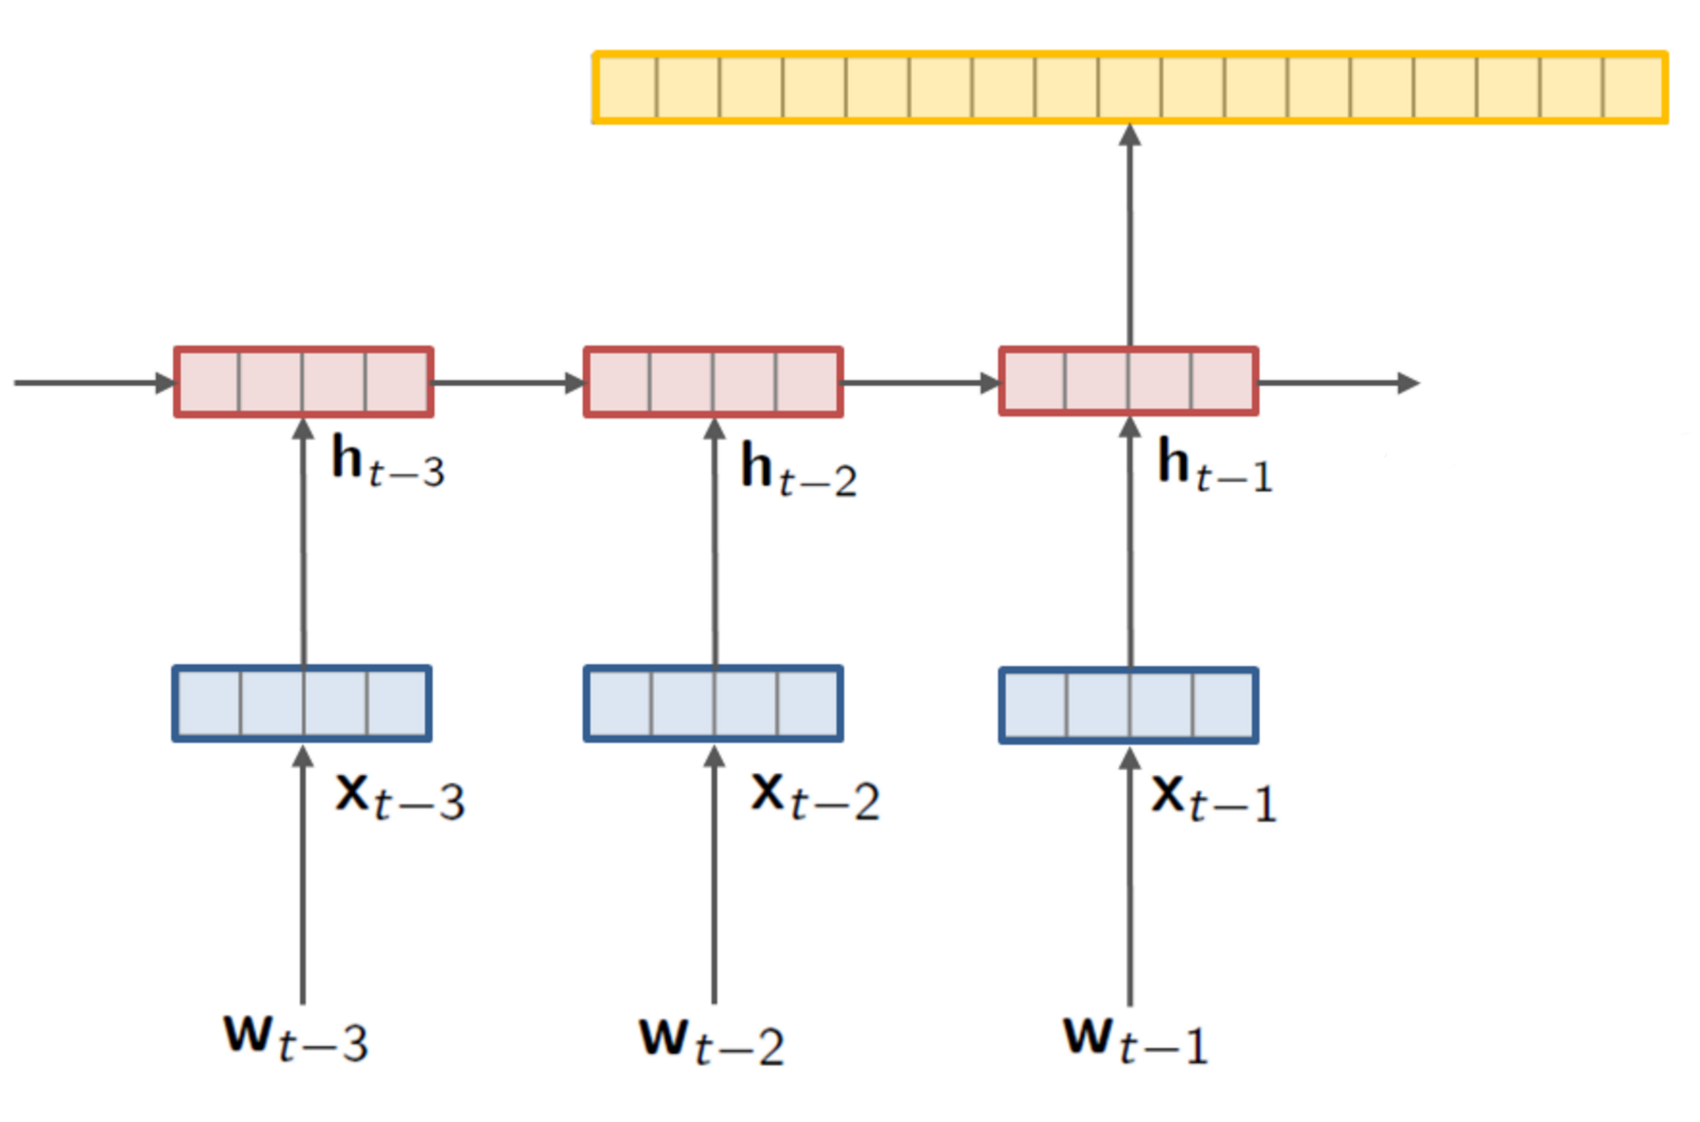
\includegraphics[width=4cm]{rnnlm6}};

    % \node[below  = of a, xshift=3cm]{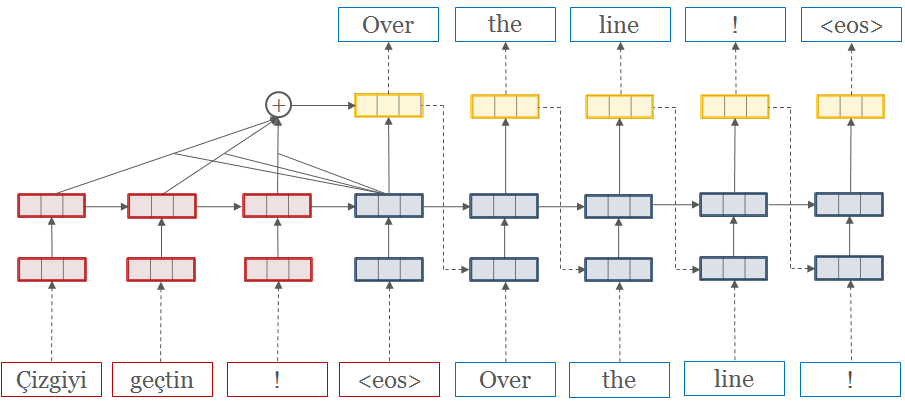
\includegraphics[width=8cm]{nmt}} ;

    % \node(b) [draw, rounded corners, minimum width=10em, minimum height=3em, below= of a]{CRF Tagging};
    % \node(c) [draw, rounded corners, minimum width=10em, minimum height=3em, below= of b]{Alignment EM};
    % \node(d) [draw, rounded corners, minimum width=10em, minimum height=3em, below= of c]{Logistic Regression};
    % \node(e) [draw, rounded corners, minimum width=10em, minimum height=3em, below= of d]{Language Modeling};
    \node [below= of e]{$\vdots$};

    \draw (aa.east) -- (a.west);
    \draw (bb.east) -- (a.west);
    \draw (cc.east) -- (a.west);
    \draw (dd.east) -- (a.west);
    \draw (ee.east) -- (a.west);
}

  \end{tikzpicture}
}


\end{center}
\end{frame}


% \begin{frame}

%   % Application pictures
% \end{frame}

% \begin{frame}{Text Generation}

%   \[ \argmax_{y_{1:T}} f(y_{1:T} ; x, \theta)\]

% \end{frame}

% \begin{frame}{Machine Learning for Natural Language}
%   What types of models get used for this equation?


%   \[\argmax_{y_{1:T}} \alert{f}(y_{1:T}, x; \alert{\theta}) \]

% \end{frame}


% \begin{frame}
%   \begin{center}
%     
\includegraphics[width=3cm]{OpenNMT}
%   \end{center}

%   \begin{itemize}
%   \item Collaborative open-source project started at Harvard, now self-sustaining.
%     \air
%   \item Used in production by Systran, Ubiqus, Booking.com, and others.
%     \air
%   \item Over 100 developers in France, China, Japan, Portugal, and the US.
%     \air
%   \item Designed to be research extensible to latest machine translation techniques.
%     \air

%   \item Pretrained models for translation as well as everything in this talk.
%   \end{itemize}
% \end{frame}

% \begin{frame}{OpenNMT Workshop} {Paris 2018}
%   \begin{center}
%     \hspace*{-9cm}\includegraphics[height=0.5\textheight]{opennmtpanaram.jpg}
%   \end{center}
% \end{frame}


% \begin{frame}{Performance}

% \end{frame}


% \begin{frame}

% \end{frame}

% \begin{frame}{Central}
%   % Picture
%   \begin{tikzpicture}
%     \node{};
%   \end{tikzpicture}
% \end{frame}
